\documentclass{article}
\usepackage{graphicx}
\usepackage{amsfonts}
\usepackage{amsmath}
\usepackage{amsthm}
\usepackage{bigfoot}
\usepackage{booktabs}
\usepackage{hyperref}
\usepackage{cleveref}
\usepackage{mathtools}
\usepackage{siunitx}
\usepackage{changes}

\usepackage{subcaption}
\usepackage{todonotes}
\usepackage{upgreek}
\usepackage{xcolor}

\usepackage[backend=biber,style=ieee]{biblatex}
% \addbibresource{ref.bib}

\usepackage{fullpage}
\usepackage[modulo]{lineno}
\linenumbers

\title{LLR 2026: Lab 3 Report}
\author{Valentina Schüller}
\date{\today}

\begin{document}

\maketitle

The code is available at
\url{https://github.com/valentinaschueller/LowRankMethods}.
In the report, I only cover the questions that explicitly required a
plot or discussion.
The remaining exercises are solved in the code in \verb|src/lab2.jl|.

\paragraph{Exercise 1}
It is a bit difficult to see from the plot (cf. \Cref{fig:denseSolver}).
I have added a statement to compute the number of singular values
larger or equal to \(\num{e-3}\sigma_1\) and the result at \(t=T\) is 55.
(\verb|sum(sv_plot ./ sv_plot[1] .≥ 1e-3)|)

\begin{figure}
  \centering
  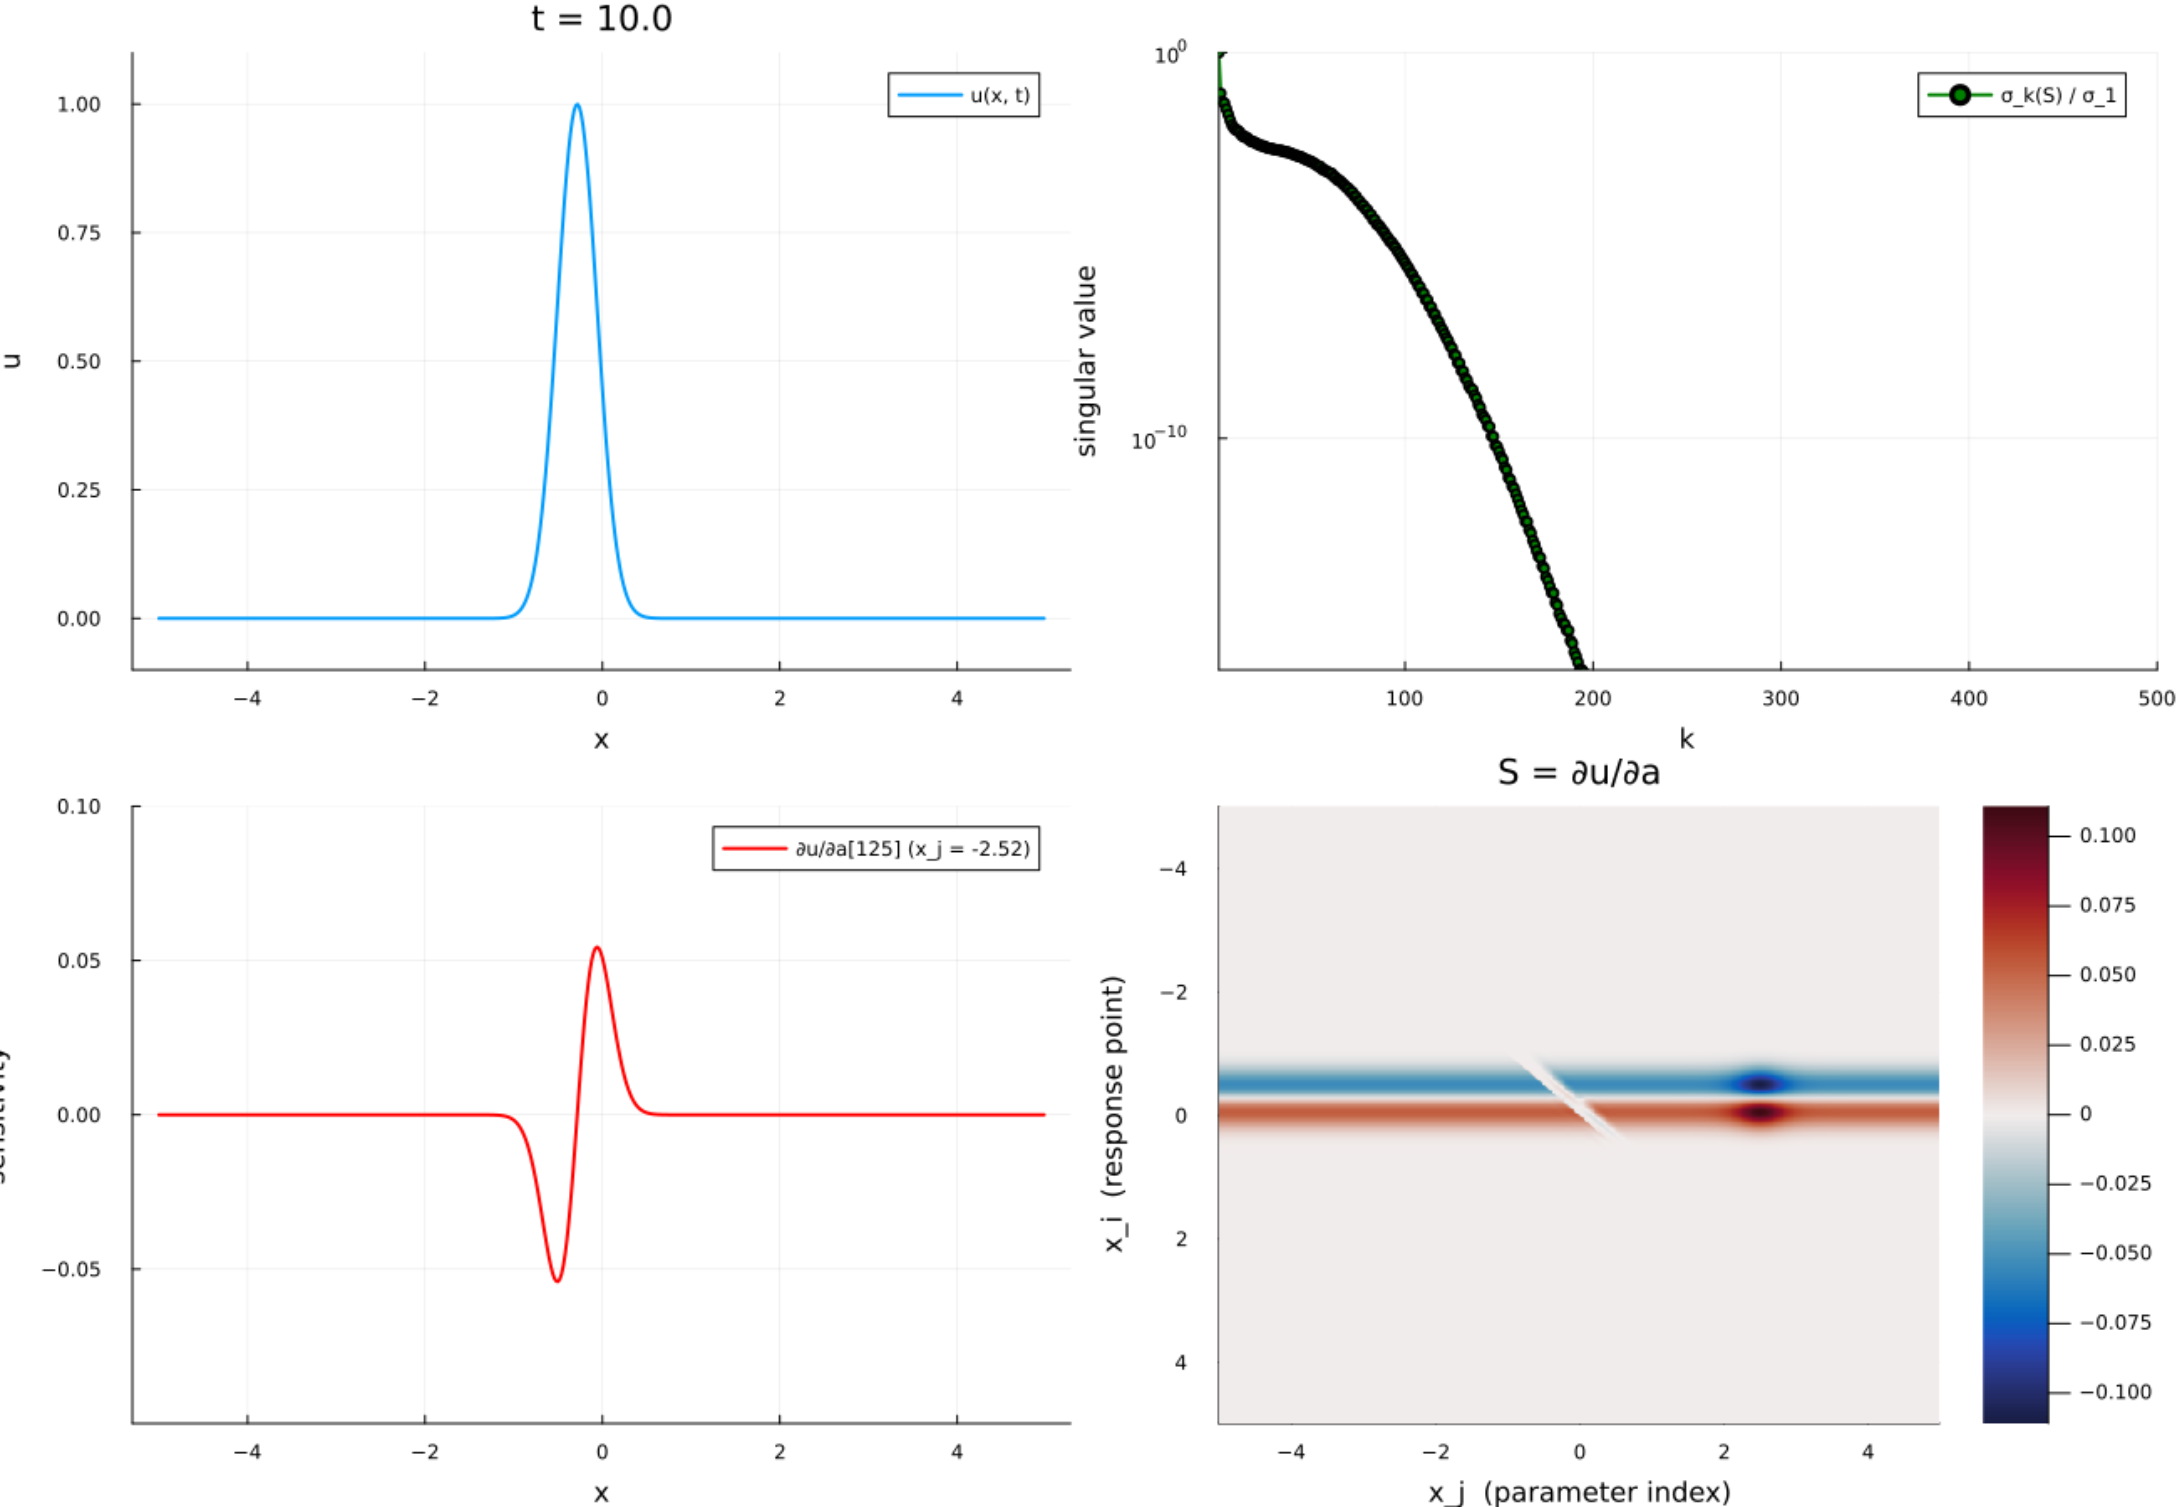
\includegraphics[width=0.8\textwidth]{figures/lab2_finalT.png}
  \caption{Dense reference solver at \(t=T\).\label{fig:denseSolver}}
\end{figure}

\end{document}
